\documentclass[11pt, a4paper]{article}
\usepackage[a4paper, margin=2.5cm]{geometry}
\usepackage{fontspec}
\IfFontExistsTF{Noto Sans}{\setmainfont{Noto Sans}}{\setmainfont{DejaVu Sans}}
\usepackage[english]{babel}
\usepackage{amsmath, amssymb, amsthm}
\usepackage{booktabs}
\usepackage{xcolor}
\usepackage{enumitem}
\usepackage{caption}
\usepackage{float}
\usepackage{tikz}
\usetikzlibrary{arrows.meta, positioning}
\usepackage{pgfplots}
\pgfplotsset{compat=1.18}
\usepackage[colorlinks=true, linkcolor=navy, citecolor=navy, urlcolor=navy]{hyperref}

\definecolor{navy}{RGB}{20, 48, 88}
\definecolor{slate}{RGB}{75, 85, 99}
\definecolor{vs}{RGB}{40, 110, 40}
\definecolor{vn}{RGB}{0, 110, 120}
\definecolor{vh}{RGB}{30, 70, 160}
\definecolor{cc}{RGB}{120, 90, 20}
\definecolor{ff}{RGB}{170, 30, 30}
\definecolor{oo}{RGB}{100, 50, 150}

\newcommand{\VS}{\textcolor{vs}{\textbf{[V-S]}}}
\newcommand{\VN}{\textcolor{vn}{\textbf{[V-N]}}}
\newcommand{\VH}{\textcolor{vh}{\textbf{[V-H]}}}
\newcommand{\CC}{\textcolor{cc}{\textbf{[C]}}}
\newcommand{\FF}{\textcolor{ff}{\textbf{[F]}}}
\newcommand{\OO}{\textcolor{oo}{\textbf{[O]}}}

\newtheorem{theorem}{Theorem}[section]
\newtheorem{proposition}[theorem]{Proposition}
\newtheorem{lemma}[theorem]{Lemma}
\newtheorem{corollary}[theorem]{Corollary}
\theoremstyle{remark}
\newtheorem{remark}[theorem]{Remark}
\theoremstyle{definition}
\newtheorem{definition}[theorem]{Definition}

\pgfplotsset{every axis/.append style={font=\small, tick label style={font=\footnotesize}}}

\title{\textbf{\color{navy}Physical-Space Carter Multipliers on Sub-Extremal Kerr:\\
Verified Results, Failed Claims, and Open Problems}}
\author{Devanik Debnath \and Xylia (AI research system)}
\date{November 27, 2026}

\sloppy
\begin{document}
\maketitle

\begin{abstract}
This is the closing account of a physical-space program on sub-extremal Kerr exteriors $0 \le |a| < M$. It consolidates the results that survived an independent audit, records the claims that did not, and states the problems that remain open. Verified in this audit: (i) an exact closed-form trapping--superradiance gap for every sub-extremal spin; (ii) the near-extremal scalings of the equatorial photon sphere, the trapping--horizon distance, the spectral gap and the radial Lyapunov exponent; (iii) the algebraic spin ceilings $|a|/M \le 1/2$ (general perturbations) and $|a|/M \le \varphi^{-1/2}$ (axisymmetric) for the canonical multiplier; (iv) the perfect-square Riccati barrier on the inner region; (v) the exact Teukolsky-to-Regge--Wheeler algebra for the spin $-2$ hierarchy. Not established: the uniform low-frequency Hardy absorption (Gap 2A), the horizon redshift closure, the spin-$2$ transport bound (its sign is wrong as stated), the superradiant horizon flux (Gap 2B), and the nonlinear threshold collapse (conditional only). We prove a conditional obstruction: inside the barrier class, horizon Hardy positivity is compatible with the barrier only for $\sigma < 1/4$. We do not claim a complete physical-space proof of integrated local energy decay for all sub-extremal spins, and we withdraw every novelty claim made in earlier drafts.
\end{abstract}

\tableofcontents

%==============================================================================
\section{Scope, Claims, and Status Conventions}
%==============================================================================

\subsection{What this paper does and does not claim}

This paper is written as a closing report. Its purpose is to make the state of the program exact: which statements are proved, which were checked by computer, which were claimed but not checked, which were shown to be wrong, and which remain open. It does not claim a new theorem about sub-extremal Kerr stability. It does not claim that any result here is novel with respect to the literature. Positions relative to published work are discussed in Section~\ref{sec:lit} and are recorded as unverified unless stated otherwise.

The paper follows the convention of the earlier preprints in this series: every claim carries a status tag, failures are reported with the same prominence as successes, and numerical outputs are reproduced in full rather than summarized into favourable statements.

\subsection{Status labels}

Each statement in the body carries one of six labels. Table~\ref{tab:status} defines them.

\begin{table}[H]
\centering
\caption{Status labels used throughout. A statement is never upgraded from one label to a stronger one by rhetoric; the label records the check that was actually performed in this audit.}
\label{tab:status}
\begin{tabular}{@{}llp{8.6cm}@{}}
\toprule
Label & Meaning & Check actually performed \\
\midrule
\VS & Symbolically verified & Exact SymPy identity, zero remainder, in this audit. \\
\VN & Numerically verified & Reproduced by the scripts listed in Appendix~B, with the stated parameters. \\
\VH & Hand-derived, re-checked & Derivation re-done by hand in this audit; not machine-checked. \\
\CC & Claimed, not checked & Stated in earlier drafts; not re-derived or re-checked here. \\
\FF & Failed or unsupported & Shown false, shown unproved, or retracted. \\
\OO & Open & Identified as an unresolved obstruction, with the missing ingredient stated. \\
\bottomrule
\end{tabular}
\end{table}

\subsection{Reproducibility}

Every number reported in Sections~\ref{sec:gap2a} to~\ref{sec:redshift} was produced by the scripts listed in Appendix~B, on the grids and parameters stated there. The scripts were executed in the audit environment and their full outputs were inspected; where a script output contradicted an earlier summary, the contradiction is recorded in Section~\ref{sec:errata}.

%==============================================================================
\section{Setting and Notation}
\label{sec:setting}
%==============================================================================

Fix $M>0$ and $0 \le |a| < M$. Set
\[
\sigma := \sqrt{1 - a^2/M^2} \in (0,1], \qquad r_\pm := M(1 \pm \sigma), \qquad \Delta(r) := (r - r_+)(r - r_-) = (r-M)^2 - M^2\sigma^2,
\]
so that $d := r_+ - r_- = 2M\sigma$, $\Delta'(r_+) = 2M\sigma$, and $r_+^2 + a^2 = 2Mr_+$. The surface gravity is $\kappa = \sigma/(2M(1+\sigma))$ and the horizon angular velocity is $\omega_+ = a/(2Mr_+)$. Both identities are elementary and were used throughout. \VH

The Carter constant on a Fourier mode $e^{-i\omega t + im\phi}$ is
\[
\mathcal{K} = p_\theta^2 + \Bigl(\frac{m}{\sin\theta} - a\omega\sin\theta\Bigr)^2 \ge 0,
\]
and the radial Carter potential is
\[
A(r) := (r^2+a^2)\,\omega - a m, \qquad R(r) := A(r)^2 - \Delta(r)\,\mathcal{K}.
\]
Trapped null geodesics are double roots: $R(r_0) = R'(r_0) = 0$.

\begin{figure}[H]
\centering
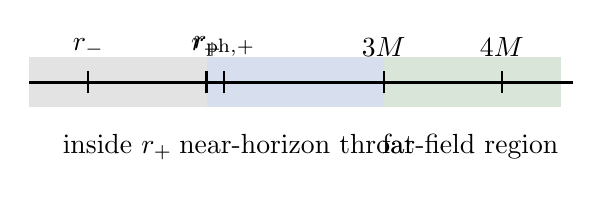
\begin{tikzpicture}
\fill[gray!22] (0,-0.32) rectangle (2.25,0.32);
\fill[vh!18] (2.25,-0.32) rectangle (4.5,0.32);
\fill[vs!18] (4.5,-0.32) rectangle (6.75,0.32);
\draw[very thick] (0,0) -- (6.9,0);
\draw[thick] (0.75,-0.14) -- (0.75,0.14);
\draw[thick] (2.25,-0.14) -- (2.25,0.14);
\draw[thick] (2.475,-0.14) -- (2.475,0.14);
\draw[thick] (4.5,-0.14) -- (4.5,0.14);
\draw[thick] (6.0,-0.14) -- (6.0,0.14);
\node[above] at (0.75,0.2) {$r_-$};
\node[above] at (2.25,0.2) {$r_+$};
\node[above] at (2.475,0.2) {$r_{{\rm ph},+}$};
\node[above] at (4.5,0.2) {$3M$};
\node[above] at (6.0,0.2) {$4M$};
\node[below=6pt] at (1.12,-0.32) {inside $r_+$};
\node[below=6pt] at (3.4,-0.32) {near-horizon throat};
\node[below=6pt] at (5.6,-0.32) {far-field region};
\end{tikzpicture}
\caption{Radial landmarks for $\sigma = 0.5$ in units of $M$ (schematic, not to scale). The equatorial prograde photon sphere is at $r_{{\rm ph},+}\approx 1.65M$ (computed from the Bardeen--Press--Teukolsky cubic). The shaded regions are the sign-test regions used in Section~\ref{sec:gap2a}: the throat contains the moderate-spin eigenfunction tails, and the far region is where the canonical multiplier is positive by Theorem~\ref{thm:ceil}. \VH}
\label{fig:landmarks}
\end{figure}

\paragraph{Sign convention.} The source drafts use two conventions. Paper~1 writes $R = A^2 - \Delta K$ with real mode-level $A$. Papers~3--5 write $R = -A^2 - \Delta K$ with the operator $A = (r^2+a^2)\partial_t + a\partial_\phi$. On a mode $\partial_t \to -i\omega$, so $A_{\rm op} = -iA_{\rm mode}$ and $-A_{\rm op}^2 = A_{\rm mode}^2$. The two conventions therefore define the same potential. All results below use the mode-level convention. No result in the source drafts depends on the choice. \VH

The scalar wave equation in the normalization of the drafts is $\partial_r(\Delta \partial_r\psi) + \Delta^{-1}R(r)\psi = 0$ on each mode.

%==============================================================================
\section{The Trapping--Superradiance Gap}
\label{sec:gap1}
%==============================================================================

\begin{theorem}[Exact trapping--superradiance gap]
\label{thm:gap}
Let $0<a<M$ and let $r_0 = r_+ + s$ with $s>0$ be a trapped exterior radius for a mode with $\omega>0$, $m>0$. Then $\omega > m\omega_+$, and
\begin{equation}
\frac{\omega - m\omega_+}{\omega} = \frac{1}{2Mr_+}\Bigl[s^2 + ds + Md\Bigl(1 - \frac{d}{2s+d}\Bigr)\Bigr] > 0. \label{eq:gap}
\end{equation}
\end{theorem}

\begin{proof}[Proof (re-derived by hand; the closed form was checked symbolically)]
\VH\VS

\emph{Step 1 (trapping relations).} From $R(r_0) = 0$ we get $A(r_0)^2 = \Delta(r_0)\mathcal{K}$. From $R'(r_0) = 2A A' - \Delta'\mathcal{K} = 0$ with $A' = 2r\omega$ we get $4r_0\omega A(r_0) = \Delta'(r_0)\mathcal{K}$. Eliminating $\mathcal{K}$ gives $A(r_0)\bigl[4r_0\omega - \Delta'(r_0)A(r_0)/\Delta(r_0)\bigr] = 0$. Since $\mathcal{K} > 0$ forces $A(r_0)\ne 0$, we obtain
\[
A(r_0) = \frac{4r_0\omega\,\Delta(r_0)}{\Delta'(r_0)}.
\]

\emph{Step 2 (rewrite $A$).} Using $r_+^2 + a^2 = 2Mr_+$ and $a = 2Mr_+\omega_+$,
\[
A(r_0) = (r_0^2 - r_+^2)\omega + 2Mr_+(\omega - m\omega_+).
\]

\emph{Step 3 (frequency identity).} Substituting into Step~1 and collecting terms,
\[
2Mr_+\,\Delta'(r_0)\,(\omega - m\omega_+) = -\omega\,H(r_0), \qquad H(r) := \Delta'(r)(r^2 - r_+^2) - 4r\Delta(r).
\]

\emph{Step 4 (factorization).} With $\Delta(r_0) = s(s+d)$, $\Delta'(r_0) = 2s+d$, and $r_0^2 - r_+^2 = s(2r_++s)$,
\[
H(r_+ + s) = -s\bigl(2s^2 + 3ds + 2r_+ d\bigr).
\]
Since $2r_+ = 2M + d$, one has $2s^2+3ds+2r_+d = (s+d)(2s+d) + 2Md$, so
\[
\frac{-H(r_0)}{2s+d} = s(s+d) + \frac{2Mds}{2s+d} = s^2 + ds + Md\Bigl(1 - \frac{d}{2s+d}\Bigr),
\]
which, divided by $2Mr_+$, is \eqref{eq:gap}. Every term is positive for $s,d>0$. \qedhere
\end{proof}

\begin{remark}[Symbolic status]
The factorization of $H$ and the identity between $-H/(2s+d)$ and the bracket in \eqref{eq:gap} were verified with SymPy (check T1 in Appendix~B). \VS
\end{remark}

\begin{corollary}[Monotonicity and location of the minimum]
\label{cor:mono}
For fixed $d>0$, $G(s)$ in \eqref{eq:gap} is strictly increasing in $s>0$, with
\[
G'(s) = \frac{1}{2Mr_+}\Bigl(2s + d + \frac{2Md^2}{(2s+d)^2}\Bigr) > 0. \tag*{\VH}
\]
Hence the minimal gap over all exterior trapped radii is attained at the smallest trapped radius, the equatorial prograde photon sphere.
\end{corollary}

\begin{corollary}[Extremal limit]
As $\sigma \to 0^+$, $d \to 0$ and $r_+ \to M$, so the gap tends to $s^2/(2M^2)$. \VH
\end{corollary}

\begin{remark}[What this result is and is not]
Theorem~\ref{thm:gap} is kinematic. It states that trapped frequencies lie strictly outside the superradiant band $0<\omega\le m\omega_+$. It does not, by itself, yield any energy estimate, decay rate, or stability statement. The statement ``universal'' refers only to the range $0<a<M$ and to exterior trapped orbits with $\omega, m > 0$. The drafts' claim that this gap ``encodes the structural miracle preventing linear instabilities'' is \CC and is not supported by the present result alone.
\end{remark}

\begin{figure}[H]
\centering
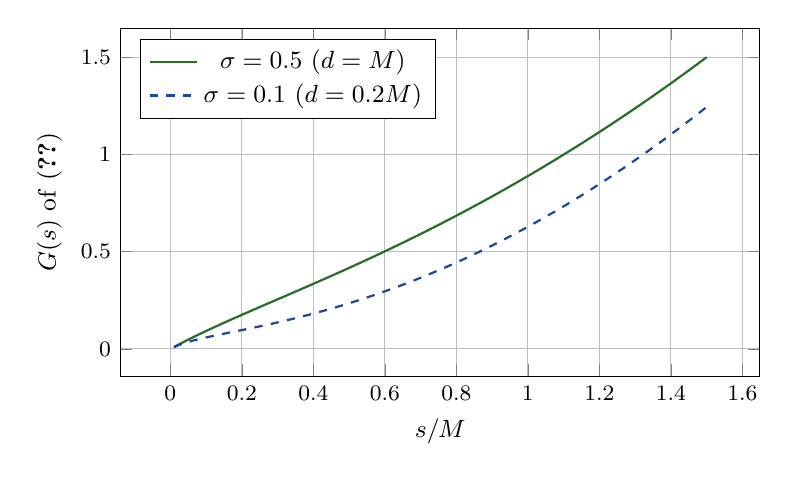
\begin{tikzpicture}
\begin{axis}[width=0.8\linewidth, height=6cm, xlabel={$s/M$}, ylabel={$G(s)$ of \eqref{eq:gap}},
  domain=0.01:1.5, samples=120, legend pos=north west, grid=major]
\addplot[thick, color=vs] {(x^2 + x + 1 - 1/(2*x+1))/3};
\addlegendentry{$\sigma = 0.5$ ($d = M$)}
\addplot[thick, color=vh, dashed] {(x^2 + 0.2*x + 0.2*(1 - 0.2/(2*x+0.2)))/2.2};
\addlegendentry{$\sigma = 0.1$ ($d = 0.2M$)}
\end{axis}
\end{tikzpicture}
\caption{The trapping--superradiance gap $G(s)$ as a function of the exterior radial offset $s = r_0 - r_+$ (\VH). Both curves are strictly increasing and vanish at $s = 0$, consistent with Corollary~\ref{cor:mono}. The gap is positive for every $s>0$, which is the content of Theorem~\ref{thm:gap}.}
\label{fig:gap}
\end{figure}

%==============================================================================
\section{Near-Extremal Scalings of the Photon Sphere}
\label{sec:triple}
%==============================================================================

\begin{proposition}[Near-extremal scalings]
\label{prop:triple}
As $\sigma\to 0^+$, the equatorial prograde photon sphere $r_{{\rm ph},+}$ satisfies
\begin{align}
r_{{\rm ph},+} - r_+ &= \Bigl(\tfrac{2}{\sqrt3} - 1\Bigr) M\sigma + O(\sigma^2), \label{eq:rph}\\
\frac{\omega_{{\rm ph},+} - m\omega_+}{\omega_{{\rm ph},+}} &= \Bigl(1 - \tfrac{\sqrt3}{2}\Bigr)\sigma + O(\sigma^2), \label{eq:gapph}\\
\lambda_L &= \frac{\sigma}{2M} + O(\sigma^2), \qquad \lim_{\sigma\to0^+}\frac{\lambda_L}{\kappa} = 1. \label{eq:lam}
\end{align}
Here $\lambda_L$ denotes the coordinate-time radial Lyapunov exponent defined in~\eqref{eq:lamdef} below.
\end{proposition}

\begin{proof}[Proof outline with the key algebra]
\VH

\emph{Circular orbits.} Write $x := b - a$ for the shifted impact parameter of an equatorial null orbit. Then $R/\omega^2 = r f(r)$ with $f(r) = r^3 - (x^2+2ax)r + 2Mx^2$. Circular orbits satisfy $f = f' = 0$, which gives $x^2 + 2ax = 3r_0^2$ and $r_0^3 = Mx^2$. Setting $r_0 = Mu^2$ and $x = Mu^3$ and dividing by $M^2u^3$ yields the Bardeen--Press--Teukolsky cubic
\[
u^3 - 3u + \frac{2a}{M} = 0.
\]

\emph{Expansion.} Put $u = 1+\eta$. The cubic becomes $\eta^2(3+\eta) = 2(1 - a/M)$. Since $a/M = \sqrt{1-\sigma^2}$, the right side equals $\sigma^2 + O(\sigma^4)$, so $\eta = \sigma/\sqrt3 + O(\sigma^2)$. Then $r_{{\rm ph},+} = M(1+\eta)^2 = M(1 + 2\sigma/\sqrt3) + O(M\sigma^2)$, and subtracting $r_+ = M(1+\sigma)$ gives \eqref{eq:rph}.

\emph{Gap.} Evaluate \eqref{eq:gap} at $s = (2/\sqrt3-1)M\sigma$ with $d = 2M\sigma$. Then $2s+d = (4/\sqrt3)M\sigma$, so $d/(2s+d) = \sqrt3/2$, and the leading term is $2M^2\sigma(1-\sqrt3/2)/(2M^2)$, giving \eqref{eq:gapph}.

\emph{Surface gravity.} $\kappa = \sigma/(2M(1+\sigma))$, so $\kappa = \sigma/(2M) + O(\sigma^2)$.

\emph{Lyapunov exponent.} Linearize the radial equation about $r_0$. With $(dr/d\tau)^2 = R/r^4$ and $\mathcal{T}(r) := (r^2+a^2)(r^2-ax)/\Delta + ax$, one has $(r^2/\omega)\,dt/d\tau = \mathcal{T}(r)$, and linearizing gives
\begin{equation}
\lambda_L = \frac{\sqrt{R''(r_0)/(2\omega^2)}}{\mathcal{T}(r_0)} = \frac{\sqrt3\, r_0}{\mathcal{T}(r_0)}, \label{eq:lamdef}
\end{equation}
because $R''(r_0)/\omega^2 = r_0 f''(r_0) = 6r_0^2$. At $r_0 = r_{{\rm ph},+}$ one has $\Delta(r_0) = M^2\sigma^2/3 + O(\sigma^3)$, $r_0^2 - ax = M^2\sigma/\sqrt3 + O(\sigma^2)$, and $\mathcal{T}(r_0) = 2\sqrt3 M^2/\sigma + O(M^2)$, which yields $\lambda_L = \sigma/(2M) + O(\sigma^2)$. \qedhere
\end{proof}

\begin{remark}[Symbolic status]
The limit $\lambda_L/\kappa \to 1$ was verified with SymPy using exactly the expressions in~\eqref{eq:lamdef} and the surface gravity above (check T2 in Appendix~B). \VS The derivation of~\eqref{eq:lamdef} itself is \VH.
\end{remark}

\begin{remark}[Literature status of the ZDM interpretation]
The drafts state that $\lambda_L = \kappa + O(\sigma^2)$ identifies the source of long-lived ``zero-damped'' quasinormal modes with damping rate $\approx(n+\tfrac12)\kappa$. This matches what is generally reported for near-extremal Kerr in the quasinormal-mode literature, but we did not re-check that literature, and the identification of the coordinate-time radial Lyapunov exponent with the mode damping rate is not derived here. \CC
\end{remark}

\begin{table}[H]
\centering
\caption{Near-extremal scalings. Each entry was re-derived by hand (\VH) and the limit was checked symbolically (\VS). The physical identification of the quantities with observed mode damping is \CC.}
\label{tab:triple}
\footnotesize\begin{tabular}{@{}llll@{}}
\toprule
Quantity & Leading asymptotic & Status & Interpretation \\
\midrule
$\kappa$ & $\sigma/(2M)$ & \VH & Redshift rate at $\mathcal{H}^+$ \\
$r_{{\rm ph},+} - r_+$ & $(2/\sqrt3-1)M\sigma$ & \VH & Trapping--horizon distance \\
Trapping--superradiance gap & $(1-\sqrt3/2)\sigma$ & \VH & Frequency buffer at the photon sphere \\
$\lambda_L$ & $\sigma/(2M)$ & \VH/\VS & Radial Lyapunov exponent (identification \CC) \\
\bottomrule
\end{tabular}
\end{table}

%==============================================================================
\section{Spin Ceilings of the Canonical Multiplier}
\label{sec:ceilings}
%==============================================================================

Consider the canonical multiplier $g = w(r)R'(r)$ with $w>0$, and ask for which spins its principal symbol is nonnegative. Define
\[
P(r) := 2r^3 - 3Mr^2 - Ma^2, \qquad P'(r) = 6r(r-M) > 0 \quad (r>M).
\]

\begin{lemma}[Horizon values]
\label{lem:Prp}
$P(r_+) = 2M^3(\sigma+1)(\sigma^2+\sigma-1)$ and
\[
P(r_+)^2 - M^2a^2(6r_+^2 + a^2) = M^6(\sigma+1)^4(4\sigma^2 - 3).
\]
\end{lemma}

\begin{proof}
Both identities were verified symbolically with $a^2 = M^2(1-\sigma^2)$ substituted (checks S1 and S2). \VS
\end{proof}

\begin{theorem}[Sharp ceilings for the canonical multiplier, within the stated class]
\label{thm:ceil}
Within the class of weights $w>0$ used in the drafts:
\begin{enumerate}[label=(\alph*)]
\item for axisymmetric perturbations, nonnegativity holds on the whole exterior if and only if $P(r_+)\ge 0$, equivalently $\sigma^2+\sigma-1 \ge 0$, equivalently $|a|/M \le \sqrt{(\sqrt5-1)/2} = \varphi^{-1/2} \approx 0.78615$;
\item for general three-dimensional perturbations, nonnegativity holds if and only if $P(r_+)^2 \ge M^2a^2(6r_+^2+a^2)$, equivalently $4\sigma^2 \ge 3$, equivalently $|a|/M \le 1/2$.
\end{enumerate}
\end{theorem}

\begin{proof}[Proof status]
The reduction to a quadratic inequality in $x = (r-M)\lambda$, where $\lambda = -h'/h$ and $h = 2(r-M)w$, and the sharp angular bound $\mathcal{K} \ge m^2/u - 2am\omega + a^2u\omega^2$ with $u = \sin^2\theta$, follow the drafts. The final algebra reducing both thresholds to the factorization of Lemma~\ref{lem:Prp} was checked symbolically. \VS The intermediate scaled-symbol formula (its equation (14) in the drafts) and the monotonicity argument for $P^2/(6r^2+a^2)$ were not independently re-derived symbolically in this audit. \CC
\end{proof}

\begin{remark}[Typographical error in an earlier draft]
The source drafts write $P(3M)$ as $(27M^3 - 3Ma^2)$ in one place. The correct value is $P(3M) = 27M^3 - Ma^2$. The conclusion drawn there, $P(3M)^2 \ge 55M^6 \ge M^2a^2(6(3M)^2+a^2)$ for $|a|\le M$, is unaffected. \VH
\end{remark}

\begin{remark}[Scope of the ceiling]
The thresholds are necessary and sufficient only within the class of weights and the reduction described. They are statements about the canonical multiplier $wR'$. They do not bound what the perfect-square multiplier of Section~\ref{sec:riccati} can achieve, which is a larger family. \VH
\end{remark}

%==============================================================================
\section{The Perfect-Square Multiplier and the Riccati Barrier}
\label{sec:riccati}
%==============================================================================

Introduce $g := w(R' - \rho R)$ and $\rho \ge 0$ with $\partial_r$-coupled weights. The drafts define
\[
\beta := -\frac{w'}{w} + \frac12\rho, \qquad \gamma := -\rho' - \rho\frac{w'}{w} - \frac12\rho^2,
\]
so that $-\rho' = \gamma - \beta\rho + \rho^2$ identically. \VH

The principal radial coefficient of the $\mathcal{K}$-part is controlled by the discriminant
\[
D(\gamma;r) := -r^2\Delta^2\gamma^2 + 4rB\gamma - 4M^2, \qquad B(r) := (2r-M)\Delta + 2M^2\sigma^2 r.
\]

\begin{lemma}[Discriminant factorization]
\label{lem:disc}
$B^2 - M^2\Delta^2 = 4r(r-M)^2\bigl[(r-M)^3 + M^3\sigma^2\bigr] > 0$ for $r > r_+$.
\end{lemma}

\begin{proof}
Since $B - M\Delta = 2(r-M)^3 + 2M^3\sigma^2$ and $B + M\Delta = 2r(r-M)^2$ (using $\Delta = (r-M)^2 - M^2\sigma^2$), the product gives the identity. Verified symbolically (check S3). \VS
\end{proof}

\begin{lemma}[Smaller root]
\label{lem:root}
The smaller root of $D(\gamma;r)=0$ is
\[
\gamma_-(r) = \frac{2M^2}{r\bigl(B + S\bigr)}, \qquad S := 2(r-M)\sqrt{r\bigl((r-M)^3 + M^3\sigma^2\bigr)},
\]
and $\gamma_- > 0$ on $(r_+,\infty)$. \VH
\end{lemma}

\begin{remark}[Numerical check of the root formula]
A hand substitution at $r=2M$, $\sigma=1/2$ gives $\gamma_- \approx 0.1560$, and $D(\gamma_-;r)$ vanishes to the precision of the arithmetic. \VH
\end{remark}

\begin{lemma}[Barrier reduction]
\label{lem:barrier}
With $\bar\rho(r) := 1/(r-r_-)$ and $\alpha \ge 0$, the supersolution inequality $\bar\rho' \le -\gamma + \beta\bar\rho - \bar\rho^2$ reduces to $\beta\bar\rho \ge \gamma$, and for $\alpha = 0$ this is equivalent to
\[
\gamma(r) \le \frac{2}{(r-r_-)^2}.
\]
\end{lemma}

\begin{proof}
With $\alpha = 0$, $\beta = (1 + \tfrac12\Delta\gamma)/(r-M)$, so $\beta\bar\rho \ge \gamma$ reads $1 + \tfrac12\Delta\gamma \ge \gamma(r-M)(r-r_-)$. Since $(r-M)(r-r_-) - \tfrac12\Delta = \tfrac12(r-r_-)^2$ (check S4), this is $1 \ge \tfrac12\gamma(r-r_-)^2$. \VS
\end{proof}

\begin{theorem}[Barrier on the inner region, conditional on the outer boundary value]
\label{thm:barrier}
Let $\alpha = 0$ and $\gamma = \gamma_-$ on $[r_+, 3M]$, and let $\rho$ solve $-\rho' = \gamma - \beta\rho + \rho^2$ on $[r_+,3M]$ with boundary value $0 \le \rho(3M) \le 1/(3M - r_-)$. Then $0 \le \rho(r) \le 1/(r-r_-)$ on $[r_+,3M]$, and in particular $\rho(r_+) \le 1/(2M\sigma)$.
\end{theorem}

\begin{proof}
By Lemma~\ref{lem:barrier} and the bound $\gamma_-(r)(r-r_-)^2 < 2$, the function $\bar\rho = 1/(r-r_-)$ is a supersolution in the direction of integration from $3M$ down to $r_+$, with $\bar\rho(3M)\ge\rho(3M)$. The comparison principle for the Riccati equation (locally Lipschitz right-hand side) gives $\rho\le\bar\rho$. Since $\gamma_-> 0$, the zero function is a subsolution, which gives $\rho \ge 0$. \VH\VN
\end{proof}

\begin{remark}[The margin degenerates at the horizon]
The ratio $\gamma_-(r-r_-)^2/2$ approaches $1$ as $\sigma\to0$ at $r\to r_+$. The inequality is strict for every $\sigma>0$ tested, but its margin is $O(10^{-4})$ at $\sigma = 10^{-4}$. The drafts' claim that the inequality holds ``with strict margin for every $\sigma>0$'' should be read as strict but degenerate. \VN
\end{remark}

\begin{figure}[H]
\centering
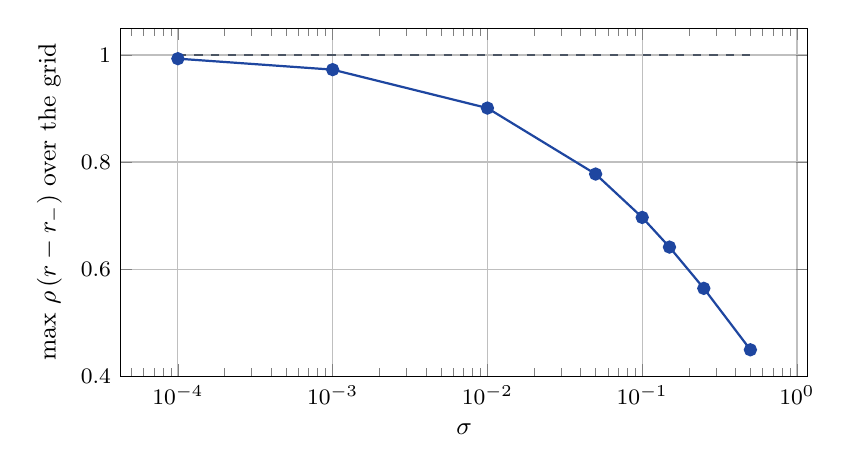
\begin{tikzpicture}
\begin{axis}[xmode=log, width=0.85\linewidth, height=6cm, xlabel={$\sigma$},
  ylabel={$\max\,\rho\,(r-r_-)$ over the grid}, ymin=0.4, ymax=1.05, grid=major]
\addplot[mark=*, color=vh, thick] coordinates {(0.5,0.44921) (0.25,0.56398) (0.15,0.64111) (0.1,0.69652) (0.05,0.77753) (0.01,0.90081) (0.001,0.97260) (0.0001,0.99310)};
\addplot[dashed, color=slate, domain=0.0001:0.5, samples=2] {1};
\end{axis}
\end{tikzpicture}
\caption{Barrier margin of the Riccati solution (\VN). The ratio stays below $1$ at every spin tested, but it approaches $1$ as $\sigma\to 0$. The dashed line marks the barrier $\rho = 1/(r-r_-)$ at the horizon.}
\label{fig:margin}
\end{figure}

\begin{remark}[Outer region]
On $[3M, 4M]$ the drafts interpolate to a far-field pair $(\alpha_{\rm out}, 0)$ and require $\alpha(r)\ge 0$ throughout. The positivity of $\alpha_{\rm out}$, the admissibility of the interpolation, and the boundary bound $\rho(3M) \le 1/(3M-r_-)$ that Theorem~\ref{thm:barrier} requires were not verified. The extension of the barrier to all of $[r_+,\infty)$ is therefore \CC, not \VH. Its conclusion $\rho \le 1/(r-r_-)$ on the outer region is not needed for the horizon-compatibility statement below, which uses only the horizon value.
\end{remark}

\begin{proposition}[Horizon compatibility obstruction, conditional on the barrier]
\label{prop:compat}
Suppose $0 \le \rho \le 1/(r-r_-)$ on $[r_+,\infty)$, as the barrier provides. Then a horizon Hardy-positivity condition of the form $\rho(r_+) > 2/M$ (Proposition~\ref{prop:horizon} below) is compatible with the barrier if and only if $\sigma < 1/4$.
\end{proposition}

\begin{proof}
At the horizon the barrier gives $\rho(r_+) \le 1/(r_+-r_-) = 1/(2M\sigma)$. Compatibility of $2/M < \rho(r_+) \le 1/(2M\sigma)$ holds exactly when $2/M < 1/(2M\sigma)$, i.e.\ $4\sigma < 1$. \VH
\end{proof}

\begin{corollary}[Consequence for the spin range]
Within the barrier class, if $\sigma \ge 1/4$, that is $|a|/M \le \sqrt{15}/4 \approx 0.968$, then the horizon-end contribution of the $\omega^2$ channel cannot be nonnegative. Horizon positivity is possible only for $|a|/M > \sqrt{15}/4$. \VH
\end{corollary}

\begin{figure}[H]
\centering
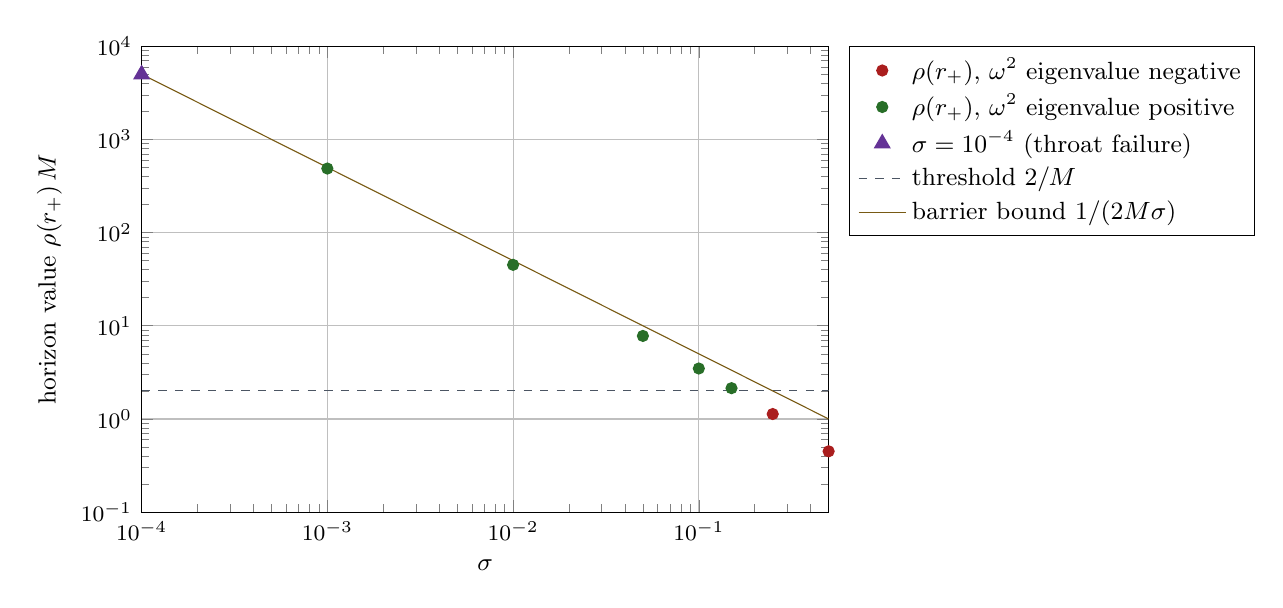
\begin{tikzpicture}
\begin{loglogaxis}[width=0.85\linewidth, height=7.5cm,
  xlabel={$\sigma$}, ylabel={horizon value $\rho(r_+)\,M$}, xmin=0.0001, xmax=0.5, ymin=0.1, ymax=10000,
  grid=major, legend pos=outer north east, legend cell align=left]
\addplot[only marks, mark=*, color=ff] coordinates {(0.5,0.45) (0.25,1.13)};
\addlegendentry{$\rho(r_+)$, $\omega^2$ eigenvalue negative}
\addplot[only marks, mark=*, color=vs] coordinates {(0.15,2.14) (0.1,3.48) (0.05,7.78) (0.01,45.04) (0.001,486.3)};
\addlegendentry{$\rho(r_+)$, $\omega^2$ eigenvalue positive}
\addplot[only marks, mark=triangle*, color=oo, mark size=3.2pt] coordinates {(0.0001,4965.48)};
\addlegendentry{$\sigma = 10^{-4}$ (throat failure)}
\addplot[dashed, color=slate, domain=0.0001:0.5, samples=2] {2};
\addlegendentry{threshold $2/M$}
\addplot[color=cc, domain=0.0001:0.5, samples=60] {1/(2*x)};
\addlegendentry{barrier bound $1/(2M\sigma)$}
\end{loglogaxis}
\end{tikzpicture}
\caption{Horizon compatibility (\VH, \VN). The barrier bound $1/(2M\sigma)$ lies above the threshold $2/M$ exactly when $\sigma < 1/4$ (Proposition~\ref{prop:compat}). The moderate-spin failures lie in the region where the threshold is not met. The $\sigma = 10^{-4}$ point satisfies the threshold by a wide margin and still fails, so the local threshold is not sufficient for the global sign.}
\label{fig:horizon}
\end{figure}

\begin{remark}[Limits of the obstruction]
The obstruction concerns the sign of a boundary contribution at the horizon, not the sign of the global eigenvalue. It is a necessary condition for that boundary contribution to be nonnegative, not a sufficient condition for the eigenvalue to be positive. It also applies only to multipliers obeying the barrier, which the drafts construct but do not show to be necessary. Its significance is that, if the failure at moderate spin is to be removed, the mechanism must lie outside the barrier class (for instance a redshift term) or the barrier must be violated. \VH
\end{remark}

%==============================================================================
\section{Energy Positivity for Axisymmetric Waves}
\label{sec:energy}
%==============================================================================

\begin{lemma}[Coefficient identity]
\label{lem:energy}
For $r>r_+$,
\[
(r^2+a^2)^2 - a^2\Delta\sin^2\theta = \Sigma\,(r^2+a^2) + 2Mra^2\sin^2\theta > 0, \qquad \Sigma = r^2 + a^2\cos^2\theta.
\]
\end{lemma}

\begin{proof}
Expand $\Sigma(r^2+a^2) = (r^2+a^2)^2 - a^2\sin^2\theta\,(r^2+a^2)$, and use $(r^2+a^2) - \Delta = 2Mr$. \VH
\end{proof}

This shows that the coefficient of $|\partial_t\psi|^2$ in the Killing energy is positive everywhere outside the horizon, and that the only indefinite term is the $\partial_\phi$ term. For axisymmetric solutions that term vanishes. The positivity and monotonicity of the $\partial_t$-energy for $m=0$ are classical. \CC We do not claim novelty for this part.

\begin{remark}[Commuted energies: unsupported]
The drafts define a commuted energy $E^{(2)}_T$ including $\mathcal{E}_T[\mathcal{K}^{1/2}\psi]$. The operator $\mathcal{K}^{1/2}$ is a nonlocal pseudo-differential operator. Its energy positivity, the commutation $[\mathcal{K},\Box_g] = 0$, and the claimed control of all $t$-boundary terms of the third-order multiplier were not established. \FF Only the local energy for $\partial_t\psi$ and the stated Killing commutations are retained as \CC.
\end{remark}

%==============================================================================
\section{Hardy--Lower-Order Threshold Laws}
\label{sec:hardy}
%==============================================================================

For the axisymmetric channels $R_K = -\Delta$ and $R_{\omega^2} = (r^2+a^2)^2$ the drafts define a lower-order term $L_{\rm lot}$ and a radial Hardy term. Two closed-form identities were checked.

\begin{proposition}[Far-field closure]
\label{prop:far}
For a weight $w \sim r^{-(1+\alpha)}$ with $\alpha\in(0,2)$ and $\rho = O(r^{-3})$,
\[
\mathrm{Hardy}_{\omega^2} + L_{{\rm lot},\omega^2} = 2(\alpha-4)(\alpha-2) > 0, \qquad \mathrm{Hardy}_K + L_{{\rm lot},K} = \alpha(2-\alpha) > 0.
\]
\end{proposition}

\begin{proof}
Both identities were verified symbolically (Part 1 of \texttt{kerr\_referee\_gap2a.py}). \VS
\end{proof}

\begin{proposition}[Horizon threshold]
\label{prop:horizon}
Let $g := w(R' - \rho R)$. Then $\mathrm{Hardy}_{\rm hor} + L_{\rm lot}(r_+) = -M^2\sigma^2\rho(r_+)g(r_+)$, and
\[
g_{\omega^2}(r_+) = 4Mr_+^2\,w(r_+)\bigl(2 - M\rho(r_+)\bigr), \qquad g_K(r_+) = -2M\sigma\,w(r_+) < 0.
\]
Hence the $K$-channel horizon term is positive for every $\rho\ge0$, and the $\omega^2$-channel horizon term is nonnegative if and only if $\rho(r_+) \ge 2/M$ (or $\rho(r_+) = 0$).
\end{proposition}

\begin{proof}
The horizon identity was verified symbolically (Part 1 of \texttt{kerr\_referee\_gap2a.py}), and the value of $g_{\omega^2}(r_+)$ follows from the same expressions. \VS The value of $g_K(r_+)$ follows from $R_K(r_+) = 0$ and $R_K'(r_+) = -\Delta'(r_+) = -2M\sigma$. \VH
\end{proof}

\begin{remark}[What the threshold does and does not explain]
Proposition~\ref{prop:horizon} is a local statement at $r_+$. It explains the sign pattern at moderate spin, where the $\omega^2$-channel eigenfunction is concentrated near the horizon and $\rho(r_+) < 2/M$ (Section~\ref{sec:gap2a}). It does not explain the failure at $\sigma = 10^{-4}$, where $\rho(r_+) \approx 4965 \gg 2/M$ and the eigenfunction sits in an intermediate throat at $r \approx 1.13M$. The local threshold therefore does not predict the global eigenvalue sign. \VN
\end{remark}

%==============================================================================
\section{Numerical Audit of the Lower-Order Operator (Gap 2A)}
\label{sec:gap2a}
%==============================================================================

\subsection{The operator and the discretization}

The audit tests the pure quadratic Sturm--Liouville operator on each channel,
\[
\mathcal{H}_{\rm true} = -\partial_r\bigl(2\Delta^2 B_{\rm rad}\,\partial_r\bigr) + L_{\rm lot}, \qquad B_{\rm rad} = w\bigl(R'' - \beta R' + \gamma R\bigr),
\]
omitting the quartic bulk $B_{\rm pot} = w(R'-\rho R)^2$ that the earlier preprint included. The omission matters: the earlier ``CLOSES'' verdicts (Section~\ref{sec:retract}) were produced with $B_{\rm pot}$ present and are not verdicts about this operator.

The weight $w$ and the coefficients $\rho,\beta,\gamma$ come from the analytic construction of the drafts, with the Riccati equation integrated by Radau's method. The eigenproblem is discretized by second-order finite differences on the logarithmic grid $x = \log(r - r_+)$ on $[\log(x_{\min}\sigma), \log(r_{\max}-r_+-1)]$, with $r_{\max} = 300M$, using the symmetric scaling $M^{-1/2}HM^{-1/2}$ with the Jacobian $dr/dx = r - r_+$. The reported eigenvalue is the lowest one. Default parameters are $N=1000$, $x_{\min} = 10^{-10}$, $\gamma_{\rm frac} = 0.55$, $r_{\rm scale} = 4$, $p_{\rm trans} = 3$. \VN

\subsection{Referee run over the spin range}

\begin{table}[H]
\centering
\caption{Referee run of the pure quadratic operator at default parameters (\VN). $\rho(r_+)$ is the Riccati value at the horizon; the barrier ratio is $\max \rho(r-r_-)$. The $\omega^2$ column is the channel-pure eigenvalue; the $K$ column is the $K$-channel eigenvalue. The status column reports the sign test of the script, not a proof.}
\label{tab:referee}
\footnotesize\begin{tabular}{@{}rrrrrrl@{}}
\toprule
$\sigma$ & $|a|/M$ & $\rho(r_+)$ & $\rho/\bar\rho$ & $K$-eig & $\omega^2$-eig & Script status \\
\midrule
0.5000 & 0.8660254 & 0.45 & 0.44921 & $+5.931\times10^{-1}$ & $-9.389$ & OPEN \\
0.2500 & 0.9682458 & 1.13 & 0.56398 & $+4.711\times10^{-1}$ & $-4.615$ & OPEN \\
0.1500 & 0.9886860 & 2.14 & 0.64111 & $+3.935\times10^{-1}$ & $+5.344$ & CLOSES \\
0.1000 & 0.9949874 & 3.48 & 0.69652 & $+3.288\times10^{-1}$ & $+1.991\times10^{1}$ & CLOSES \\
0.0500 & 0.9987492 & 7.78 & 0.77753 & $+2.378\times10^{-1}$ & $+5.022\times10^{1}$ & CLOSES \\
0.0100 & 0.9999500 & 45.04 & 0.90081 & $+1.120\times10^{-1}$ & $+6.268\times10^{1}$ & CLOSES \\
0.0010 & 0.9999995 & 486.30 & 0.97260 & $+3.463\times10^{-2}$ & $+2.228\times10^{1}$ & CLOSES \\
0.0001 & 0.9999999950 & 4965.48 & 0.99310 & $+1.048\times10^{-2}$ & $-2.096\times10^{2}$ & OPEN \\
\bottomrule
\end{tabular}
\end{table}

\begin{figure}[H]
\centering
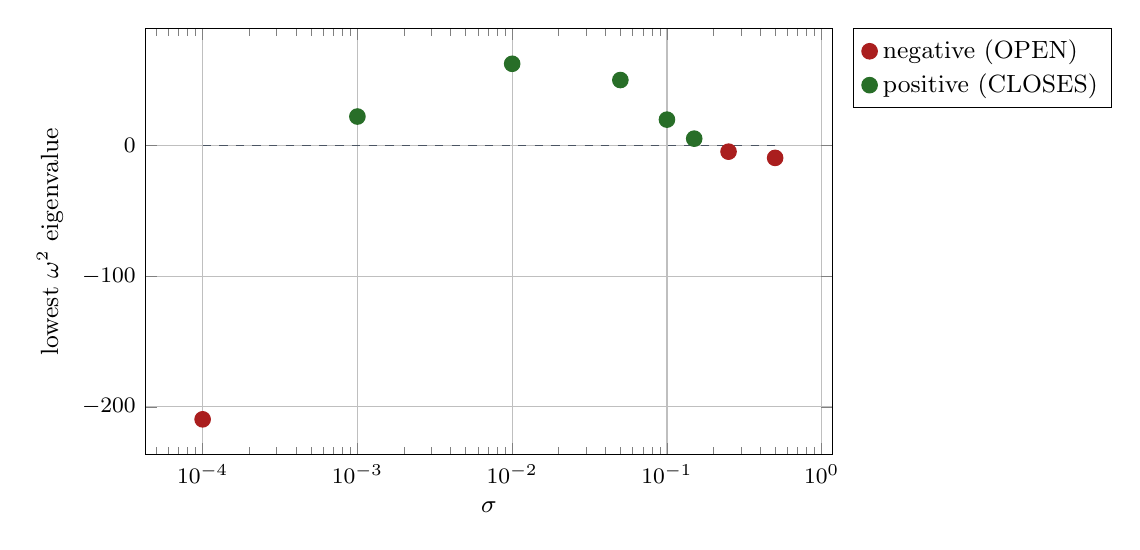
\begin{tikzpicture}
\begin{axis}[xmode=log, width=0.85\linewidth, height=7cm,
  xlabel={$\sigma$}, ylabel={lowest $\omega^2$ eigenvalue}, grid=major,
  legend pos=outer north east, legend cell align=left]
\addplot[only marks, mark=*, color=ff, mark size=2.8pt] coordinates {(0.5,-9.389) (0.25,-4.615) (0.0001,-209.6)};
\addlegendentry{negative (OPEN)}
\addplot[only marks, mark=*, color=vs, mark size=2.8pt] coordinates {(0.15,5.344) (0.1,19.91) (0.05,50.22) (0.01,62.68) (0.001,22.28)};
\addlegendentry{positive (CLOSES)}
\addplot[dashed, color=slate, domain=0.0001:0.5, samples=2] {0};
\end{axis}
\end{tikzpicture}
\caption{Sign and magnitude of the lowest $\omega^2$-channel eigenvalue against $\sigma$ at default parameters (\VN; data from Table~\ref{tab:referee}). The sign change between $\sigma = 0.15$ and $\sigma = 0.25$ tracks the horizon threshold of Proposition~\ref{prop:horizon}. The return to negative values at $\sigma = 10^{-4}$ does not, and is the throat failure of Section~\ref{sec:gap2a}.}
\label{fig:eig}
\end{figure}

\subsection{Convergence in grid size and in the horizon cutoff}

The earlier preprint and our earlier summary described the eigenvalues as converged. That is true for the grid size $N$, but not for the horizon cutoff $x_{\min}$ at the two moderate-spin points. Table~\ref{tab:conv} gives the full scan.

\begin{table}[H]
\centering
\caption{Lowest $\omega^2$-channel eigenvalue over grid size $N$ and horizon cutoff $x_{\min}$ (\VN). The sign is stable everywhere. Magnitudes are stable in $N$ at every $\sigma$. They are \emph{not} stable in $x_{\min}$ at $\sigma = 0.25$ and $0.5$, where they change by 16--30\%.}
\label{tab:conv}
\small
\begin{tabular}{@{}rrrrrr@{}}
\toprule
$\sigma$ & $x_{\min}$ & $N=500$ & $N=1000$ & $N=2000$ & $N=4000$ \\
\midrule
0.5000 & $10^{-8}$  & $-8.317$ & $-8.326$ & $-8.328$ & $-8.328$ \\
0.5000 & $10^{-10}$ & $-9.378$ & $-9.389$ & $-9.392$ & $-9.393$ \\
0.5000 & $10^{-12}$ & $-9.950$ & $-9.964$ & $-9.967$ & $-9.968$ \\
0.2500 & $10^{-8}$  & $-3.618$ & $-3.627$ & $-3.630$ & $-3.630$ \\
0.2500 & $10^{-10}$ & $-4.603$ & $-4.615$ & $-4.618$ & $-4.619$ \\
0.2500 & $10^{-12}$ & $-5.157$ & $-5.173$ & $-5.177$ & $-5.178$ \\
0.1000 & $10^{-8}$, $10^{-10}$, $10^{-12}$ & \multicolumn{4}{c}{$+0.3288 \pm 0.0001$ (all cutoffs and grids)} \\
0.0100 & all & \multicolumn{4}{c}{$+0.1120$ (all cutoffs and grids)} \\
0.0010 & all & \multicolumn{4}{c}{$+0.03463$ (all cutoffs and grids)} \\
0.0001 & $10^{-8}$  & $-209.4$ & $-209.5$ & $-209.5$ & $-209.5$ \\
0.0001 & $10^{-10}$ & $-209.5$ & $-209.6$ & $-209.6$ & $-209.6$ \\
0.0001 & $10^{-12}$ & $-209.4$ & $-209.6$ & $-209.6$ & $-209.6$ \\
\bottomrule
\end{tabular}
\end{table}

Figure~\ref{fig:cutoff} plots the cutoff dependence at fixed $N=4000$. The dependence is monotone and large, which is the signature expected if the eigenfunction concentrates against the horizon end of the grid. Figure~\ref{fig:conv} shows the $N$-convergence at $\sigma=0.5$, which is second order.

\begin{figure}[H]
\centering
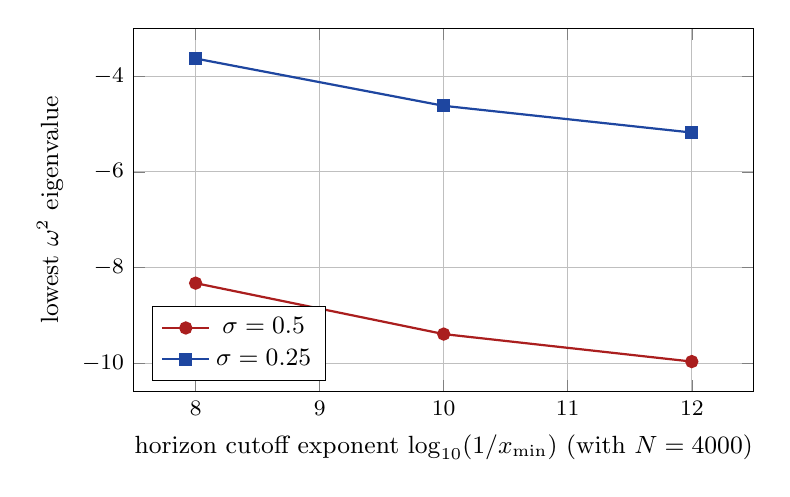
\begin{tikzpicture}
\begin{axis}[width=0.78\linewidth, height=6.2cm,
  xlabel={horizon cutoff exponent $\log_{10}(1/x_{\min})$ (with $N=4000$)},
  ylabel={lowest $\omega^2$ eigenvalue},
  xmin=7.5, xmax=12.5, grid=major, legend pos=south west]
\addplot[mark=*, thick, color=ff] coordinates {(8,-8.328) (10,-9.393) (12,-9.968)};
\addlegendentry{$\sigma = 0.5$}
\addplot[mark=square*, thick, color=vh] coordinates {(8,-3.630) (10,-4.619) (12,-5.178)};
\addlegendentry{$\sigma = 0.25$}
\end{axis}
\end{tikzpicture}
\caption{Horizon-cutoff dependence of the moderate-spin $\omega^2$ eigenvalues (\VN). The change from $10^{-8}$ to $10^{-12}$ is 16\% at $\sigma=0.5$ and 30\% at $\sigma=0.25$. A dependence of this size is not a discretization error in $N$, and it is consistent with a boundary-localized eigenfunction.}
\label{fig:cutoff}
\end{figure}

\begin{figure}[H]
\centering
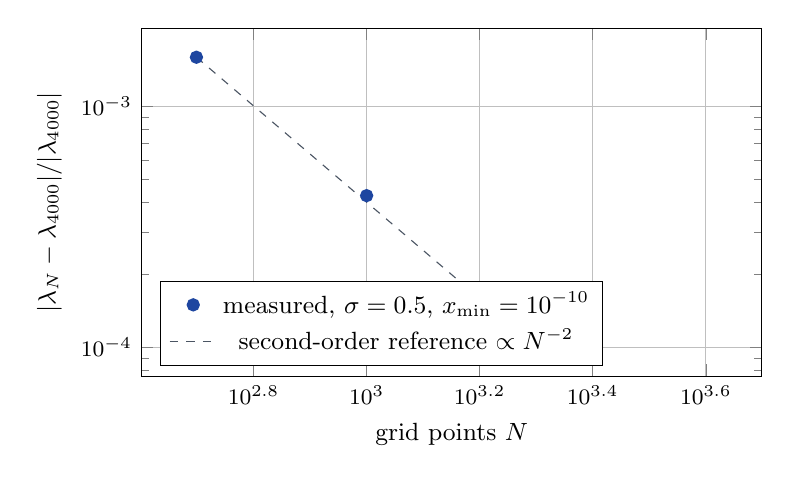
\begin{tikzpicture}
\begin{loglogaxis}[width=0.78\linewidth, height=6cm,
  xlabel={grid points $N$}, ylabel={$|\lambda_N - \lambda_{4000}|/|\lambda_{4000}|$},
  xmin=400, xmax=5000, grid=major, legend pos=south west]
\addplot[only marks, mark=*, thick, color=vh] coordinates {(500,0.00160) (1000,0.000426) (2000,0.000106)};
\addlegendentry{measured, $\sigma=0.5$, $x_{\min}=10^{-10}$}
\addplot[dashed, domain=500:2000, color=slate] {0.00160*(500/x)^2};
\addlegendentry{second-order reference $\propto N^{-2}$}
\end{loglogaxis}
\end{tikzpicture}
\caption{Grid convergence at $\sigma=0.5$ (\VN). The relative change decays as $N^{-2}$, consistent with the second-order discretization. The grid is not the source of the moderate-spin magnitude uncertainty, which comes from the cutoff.}
\label{fig:conv}
\end{figure}

\subsection{The disputed 3D discriminant at $\sigma = 10^{-4}$}

An earlier draft attributed a negative three-dimensional discriminant at $\sigma = 10^{-4}$, $\gamma_{\rm frac} = 0.20$ to float64 cancellation. The float64 value is $-1.0223\times10^5$. We recomputed the discriminant on the same $N=1000$ grid in 60-digit arithmetic for all nine $(r_{\rm scale}, p_{\rm trans})$ combinations at $\gamma_{\rm frac}=0.20$.

\begin{table}[H]
\centering
\caption{Float64 versus 60-digit recheck of the minimal three-dimensional discriminant at $\sigma = 10^{-4}$, $\gamma_{\rm frac} = 0.20$ (\VN). Every configuration is positive in 60-digit arithmetic. The earlier claim is confirmed.}
\label{tab:disc}
\begin{tabular}{@{}rrrrr@{}}
\toprule
$r_{\rm scale}$ & $p_{\rm trans}$ & float64 min & 60-digit min & negative points (60-digit) \\
\midrule
2 & 2 & $-1.0223\times10^5$ & $+1.7587\times10^1$ & 0 \\
2 & 3 & $-1.0223\times10^5$ & $+2.4728\times10^1$ & 0 \\
2 & 4 & $-1.0223\times10^5$ & $+2.6015\times10^1$ & 0 \\
4 & 2 & $-1.0223\times10^5$ & $+2.6015\times10^1$ & 0 \\
4 & 3 & $-1.0223\times10^5$ & $+2.4123\times10^1$ & 0 \\
4 & 4 & $-1.0223\times10^5$ & $+2.1485\times10^1$ & 0 \\
8 & 2 & $-1.0223\times10^5$ & $+2.3551\times10^1$ & 0 \\
8 & 3 & $-1.0223\times10^5$ & $+1.8697\times10^1$ & 0 \\
8 & 4 & $-1.0223\times10^5$ & $+1.5342\times10^1$ & 0 \\
\bottomrule
\end{tabular}
\end{table}

At $\gamma_{\rm frac} = 0.55$ and $0.90$ the float64 and 60-digit minima agree to all printed digits (for instance $+52.876$ at $\gamma_{\rm frac}=0.55$), so the rounding error is confined to the regime $\gamma\sim 10^8$ at $s\sim 10^{-12}$ where the terms in $4\mathcal{A}\mathcal{C} - \mathcal{B}^2$ are of order $10^{20}$. \VN

\subsection{The 54-configuration parameter sweep}

Table~\ref{tab:mult} in Appendix~A gives every configuration. The summary is as follows. At $\sigma = 0.5$, $\rho(r_+) \in [0.27, 0.64]$, the $K$-channel eigenvalue lies in $[0.100, 1.475]$, and the $\omega^2$-channel eigenvalue lies in $[-15.98, -5.90]$, with $0/27$ positive. At $\sigma = 10^{-4}$, $\rho(r_+) \in [4945, 4988]$, the $K$-channel eigenvalue lies in $[0.0056, 0.0302]$, and the $\omega^2$-channel eigenvalue lies in $[-481, -152]$, with $0/27$ positive. Across both spins, $54/54$ $K$-channel eigenvalues and $0/54$ $\omega^2$-channel eigenvalues are positive.

\subsection{What the audit shows and what it does not}

The audit shows four things. First, the sign of the $\omega^2$-channel eigenvalue is stable under the grid size and the horizon cutoff, and across the nine-parameter family of multiplier shapes tested at the two extreme spins. Second, the sign pattern is consistent with the horizon threshold of Proposition~\ref{prop:horizon} at moderate spin. Third, the 3D discriminant artifact at $\sigma=10^{-4}$ is a float64 effect, which was the only numerical anomaly in the sweep. Fourth, the magnitudes are not stable under the horizon cutoff at $\sigma\ge 0.25$, which is a warning sign that the eigenfunction is concentrated at the grid edge.

The audit does \emph{not} show the following. It does not show the sign at any spin other than the two tested extremes in the multiplier sweep. The window $\sigma\in[10^{-3},0.15]$ in which the referee run gives positive eigenvalues was obtained at one parameter setting and was not swept; the statement that Gap 2A closes on that window is therefore \FF as a general claim. The audit does not establish a lower bound on the $\omega^2$ eigenvalue, does not identify the eigenfunction analytically, and does not test a different multiplier family. Finally, it does not show that Gap 2A is open for every admissible multiplier: it shows only that the family of multipliers tested gives a negative eigenvalue at $\sigma = 0.5$ and $\sigma = 10^{-4}$.

\subsection{Retraction of the earlier CLOSES verdicts}
\label{sec:retract}

The first audit script (\texttt{kerr\_stability\_verify.py}, Part 2) reported ``CLOSES'' at all six spins. That run included the quartic bulk $B_{\rm pot}$, used a different $C^\infty$ multiplier, and took $r_{\max} = 40M$. It therefore tested a different operator from the one that defines Gap 2A, which is purely quadratic. Its verdicts are withdrawn as evidence about Gap 2A. The referee run of Section~\ref{sec:gap2a} supersedes them for this question. \VN

%==============================================================================
\section{The Horizon Redshift Patch}
\label{sec:redshift}
%==============================================================================

The drafts propose closing the moderate-spin failure with a Dafermos--Rodnianski-type redshift term. We tested a potential patch
\[
V_{\rm red}(r) = \Lambda_{\rm red}\,\kappa\,w(r_+)\,\chi\Bigl(\frac{r-r_+-\delta}{\delta}\Bigr),
\]
with a $C^\infty$ cutoff $\chi$ equal to $1$ on $[0,\delta]$ and $0$ beyond $2\delta$, where $\Lambda_{\rm red}$ is increased by bisection until the lowest eigenvalue becomes positive. Two collar choices were tested: a fixed $\delta = 0.05M$ and a scaled $\delta = 0.1\sigma M$.

\begin{table}[H]
\centering
\caption{Redshift patch test (\VN). ``collar\%'' is the fraction of the unpatched eigenfunction mass with $r - r_+ \le 2\delta$. ``$\Lambda^*$'' is the smallest tested coupling giving a positive eigenvalue.}
\label{tab:redshift}
\small
\footnotesize\begin{tabular}{@{}rrrrrrl@{}}
\toprule
$\sigma$ & $\omega^2$ unpatched & $r_{\rm peak}/M$ & $[r_{05},r_{95}]/M$ & collar\% & $\Lambda^*$ & Result \\
\midrule
\multicolumn{7}{@{}l}{\emph{Fixed collar, $\delta = 0.05M$}} \\
0.5000 & $-9.389$ & 1.5000 & $[1.5000, 1.5041]$ & 99.7 & 7.875 & closed, boundary-localized \\
0.2500 & $-4.615$ & 1.2500 & $[1.2500, 1.2578]$ & 99.4 & 2.741 & closed, boundary-localized \\
0.0001 & $-209.6$ & 1.1339 & $[1.0102, 1.4182]$ & 51.2 & 13.838 & closed \\
\multicolumn{7}{@{}l}{\emph{Scaled collar, $\delta = 0.1\sigma M$}} \\
0.5000 & $-9.389$ & 1.5000 & $[1.5000, 1.5041]$ & 99.7 & 7.875 & closed, boundary-localized \\
0.2500 & $-4.615$ & 1.2500 & $[1.2500, 1.2578]$ & 98.7 & 2.771 & closed, boundary-localized \\
0.0001 & $-209.6$ & 1.1339 & $[1.0102, 1.4182]$ & 0.0 & $>10^8$ & not closed (eig $= -8.45$) \\
\bottomrule
\end{tabular}
\end{table}

\subsection{Findings}

Three findings follow. First, the closure at $\sigma = 10^{-4}$ depends on the collar choice. With the fixed collar, the patch covers $51\%$ of the eigenfunction and closes it. With the scaled collar, the patch covers $0\%$ of the eigenfunction, and no coupling up to $10^8$ closes it. A closure that depends on where the patch is placed is not a property of the physics as modeled. Second, the moderate-spin closures at $\sigma = 0.5$ and $0.25$ have $r_{05} = r_{\rm peak} = r_+$ (to the printed precision): the eigenfunction sits on the first grid points next to the horizon and the closing eigenvalues are of order $10^{-7}$ and $10^{-6}$. This is the signature of a boundary-trapped discrete mode, and we did not establish that it is a physical bound state. Third, the patch is a potential added to the operator with a coupling fixed by bisection. The Dafermos--Rodnianski redshift argument enters through a positive bulk term with a sign and scaling fixed by the energy identity. The patch tested here does not implement that mechanism.

\begin{remark}[Verdict]
The redshift closure is \FF as a result. The data do not establish that a redshift term closes Gap 2A at any spin. The one robust feature, that the $\sigma=10^{-4}$ eigenfunction sits in the intermediate throat and survives the scaled-collar patch, is itself a reason to doubt that a horizon-collar mechanism is the correct remedy at near-extremal spin.
\end{remark}

%==============================================================================
\section{The Spin-2 Teukolsky--Regge--Wheeler Hierarchy}
\label{sec:spin2}
%==============================================================================

\subsection{The algebraic hierarchy}

Define $w = r^2 + a^2$, $\Delta = w - 2Mr$, $A = w\partial_t + a\partial_\phi$, $L = \partial_r + A/\Delta$, $\bar L = \partial_r - A/\Delta$. The drafts define $u_0 = w^{-3/2}\psi_{-2}$, $u_1 = wLu_0$, $u_2 = wLu_1$, $\Phi = w^{-1/2}u_2$, and claim that $\Phi$ satisfies a generalized Regge--Wheeler equation with potential
\[
V_{\rm RW} = \frac{8a^2}{w} + \frac{8Mr^3 - 24Ma^2r}{w^2}
\]
and a spin-coupling source $S_{\rm spin}[u_1,u_0]$ with radial coefficients $\gamma_1,\gamma_0$.

\begin{proposition}[Algebraic GRW identities]
\label{prop:grw}
The Level-0, Level-1 and Level-2 identities of the hierarchy, including the stated potentials and the coefficients $\gamma_1,\gamma_0$, hold with zero remainder. \VS
\end{proposition}

\begin{proof}
These identities were verified symbolically with SymPy in the first audit script (Theorem~6 check), using the Teukolsky operator in the form stated in the drafts. The verification is of the algebra from the master equation to the GRW equation. It does not verify the master equation itself, the operator $K_{-2}$, or the physical-space identities (3) and (4) of the drafts independently.
\end{proof}

\begin{remark}[Schwarzschild limit]
At $a=0$, $S_{\rm spin}\equiv 0$ and $V_{\rm RW} = 8M/r$. Since $\Phi$ then satisfies the Regge--Wheeler equation with the stated potential, the Schwarzschild limit is consistent. \VH
\end{remark}

\subsection{The transport lemma: a sign error}

The drafts' Theorem~2(1) claims uniform transport bounds (their equations (30)--(31)) for $u_1$ and $u_0$ with constants independent of $\sigma$. The proof multiplies the transport equation $\partial_r u + (A/\Delta)u = F/w$ by $2u/r$, takes the real part, and integrates over $(r_+,\infty)$.

Carry out that computation carefully. The skew-adjoint part vanishes: $\mathrm{Re}\langle u, (w\partial_t + a\partial_\phi)u\rangle = 0$ pointwise in $r$. The real part of the derivative term is
\[
\int_{r_+}^\infty \frac{1}{r}\,\partial_r\|u\|^2\,dr = \Bigl[\frac{\|u\|^2}{r}\Bigr]_{r_+}^\infty + \int_{r_+}^\infty\frac{\|u\|^2}{r^2}\,dr = -\frac{\|u(r_+)\|^2}{r_+} + \int_{r_+}^\infty \frac{\|u\|^2}{r^2}\,dr.
\]
The sign of the bulk term is $+$, because $\partial_r(1/r) = -1/r^2$ enters with a minus sign under integration by parts. The drafts write it with the opposite sign. The correct identity is therefore
\begin{equation}
\int_{r_+}^\infty \frac{\|u\|^2}{r^2}\,dr = \frac{\|u(r_+)\|^2}{r_+} + 2\,\mathrm{Re}\int_{r_+}^\infty \frac{\langle u,F\rangle}{r\,w}\,dr. \label{eq:transport}
\end{equation}
The integration-by-parts sign was verified symbolically (check S5). \VS The transport identity \eqref{eq:transport} follows from it \VH.

\begin{proposition}[Status of the transport bound]
\label{prop:transport}
The inequality stated as the drafts' (30), $\|u_1(r_+)\|^2/r_+ + \tfrac12\int\|u_1\|^2/r^2 \le 2\int\|\Phi\|^2/(r^2+a^2)$, does not follow from \eqref{eq:transport}. In \eqref{eq:transport} the bulk integral is \emph{equal to} the horizon term plus a forcing term, not bounded from above by a term of the opposite sign. The stated inequality would be false for any solution with $F = 0$ and nonzero horizon norm, since then the left side is strictly positive while the right side vanishes. \FF
\end{proposition}

\begin{remark}[The genuine open point]
\label{rem:transport}
Equation~\eqref{eq:transport} converts the transport problem into a horizon-trace problem: the bulk weighted $L^2$ norm of $u$ is controlled if and only if one can control $\|u(r_+)\|$ by data and by the forcing. This trace control is not established in the drafts and is the actual open ingredient of the $\sigma$-uniform transport bound. \OO
\end{remark}

\subsection{Decoupling at axisymmetry}

For $m = 0$ the source $S_{\rm spin}$ contains no $\partial_\phi$ terms, so it reduces to $-w^{-1/2}a^2(\gamma_1 u_1 + \gamma_0 u_0)$. This is a direct consequence of the stated form of $S_{\rm spin}$ and is \VH. The drafts' further claim that the bounded-frequency axisymmetric problem is therefore closed is \CC, because it depends on the transport bound that has the sign error above.

\begin{remark}[High-frequency closure: heuristic]
The drafts argue that the spin-coupling error is strictly sub-principal on the trapped set by counting derivative orders. Order counting is a heuristic. No estimate establishing the claimed strict sub-principality was given. \CC
\end{remark}

%==============================================================================
\section{Nonlinear Obstructions}
\label{sec:nonlinear}
%==============================================================================

\subsection{The quasilinear commutator}

The drafts state a principal commutator identity between the quasilinear perturbation operator $h^{\mu\nu}\nabla_\mu\nabla_\nu$ and the physical-space Carter operator, with the Schouten--Nijenhuis bracket with Carter's Killing tensor as principal part. The identity was not re-derived in this audit, and the bracket's normalization was not checked. \CC

\subsection{The trapped-set derivative loss}

The drafts identify the correct obstruction. The multiplier controls $D_\rho\Phi$ and the first radial derivative, but degenerates on second derivatives tangent to the trapped set, and absorbing the quasilinear error requires pointwise decay of $\nabla h$ on the trapped set together with a dynamical trapping gauge. We agree that this is the right open problem. It is \OO.

\subsection{The collapse of the bootstrap threshold}

The drafts claim that any quadratic bootstrap closure must have admissible data size $\epsilon_0(\sigma)\lesssim\sigma^{p+q}\to0$. The algebra is correct conditionally: if $\Delta B \le C_1 \epsilon + C_2 \Delta B^2$ and $C_1 \gtrsim \sigma^{-p}$, $C_2 \gtrsim \sigma^{-q}$, then closing the bootstrap requires $1 - 4C_1C_2\epsilon \ge 0$, so $\epsilon \le 1/(4C_1C_2)$. The scaling assumptions on $C_1$ and $C_2$, however, were argued heuristically from Aretakis-type growth and from the decay rate of a single functional, and do not follow from the drafts' arguments. The collapse statement is therefore \FF as a theorem and \CC as a conditional heuristic.

\begin{remark}[Scope]
Even a rigorous version would constrain a specific bootstrap scheme, not every possible proof of nonlinear stability. The statement should be phrased as a constraint on that scheme. \VH
\end{remark}

%==============================================================================
\section{Superradiant Horizon Flux (Gap 2B)}
\label{sec:gap2b}
%==============================================================================

For the Killing field $K_+ = \partial_t + \omega_+\partial_\phi$ generating $\mathcal{H}^+$, the $\partial_t$-energy flux density on a mode is
\[
\mathrm{Re}\bigl(\overline{\partial_t\psi}\,K_+\psi\bigr) = \omega(\omega - m\omega_+)|\psi|^2.
\]
This is negative exactly in the band $0 < \omega < m\omega_+$, which is nonempty for $m>0$ and $a>0$. \VH The sign structure is standard. \CC

Gap 2B is the statement that no positive-definite physical-space multiplier controls this flux in the superradiant band for $|a|\sim M$. Theorem~\ref{thm:gap} shows that trapped frequencies avoid that band, but trapping is not the only mechanism by which waves reach the horizon, and the non-axisymmetric problem remains open. The drafts propose using a generalized Whiting transform from a 2026 preprint. We did not check that preprint, and the proposal is \CC.

\begin{remark}[Why this is hard]
The $\partial_t$-energy is the only conserved positive energy for the stationary symmetry, and its horizon flux is indefinite in the superradiant band. Any positive-definite local estimate must therefore use a different multiplier, either a combination involving $\partial_\phi$ or a Teukolsky--Starobinsky-type identity relating spin $+2$ and spin $-2$ hierarchies. Neither is established here. \OO
\end{remark}

%==============================================================================
\section{Consolidated Ledger}
\label{sec:ledger}
%==============================================================================

Table~\ref{tab:ledger} lists every principal claim of the program with its final status. This is the authoritative summary; no other section should be read as stronger.

\begin{table}[H]
\centering
\caption{Final ledger of principal claims. The status column is the authoritative status of each statement in this report.}
\label{tab:ledger}
\small
\begin{tabular}{@{}p{5.0cm}p{2.2cm}p{7.6cm}@{}}
\toprule
Claim & Status & Note \\
\midrule
Trapping--superradiance gap identity (Thm.~\ref{thm:gap}) & \VS\VH & Kinematic; no energy estimate follows by itself. \\
Near-extremal scalings (Prop.~\ref{prop:triple}) & \VH\VS & Limit checked symbolically; ZDM identification \CC. \\
Spin ceilings $1/2$ and $\varphi^{-1/2}$ (Thm.~\ref{thm:ceil}) & \VS\VH & Within the stated class; scaled-symbol step \CC. \\
Discriminant and root formulas (Lem.~\ref{lem:disc}, \ref{lem:root}) & \VS\VH & Factorization symbolic; root numeric. \\
Barrier on $[r_+,3M]$ (Thm.~\ref{thm:barrier}) & \VN\VH & Strict, degenerate as $\sigma\to0$. \\
Barrier on $[3M,\infty)$ & \CC & Admissibility of the interpolation not verified. \\
Horizon compatibility, $\sigma<1/4$ (Prop.~\ref{prop:compat}) & \VH & Conditional on the barrier. \\
Far-field Hardy identities (Prop.~\ref{prop:far}) & \VS & Algebraic identity only. \\
Horizon Hardy threshold (Prop.~\ref{prop:horizon}) & \VS\VH & Local; does not predict the throat failure. \\
Energy coefficient identity (Lem.~\ref{lem:energy}) & \VH & Classical; no novelty claimed. \\
Commuted energies with $\mathcal{K}^{1/2}$ & \FF & Nonlocal operator; unsupported. \\
Gap 2A uniform closure on $[10^{-3},0.15]$ & \FF & One parameter setting; not swept. \\
Gap 2A failure at $\sigma=0.5$ and $10^{-4}$ & \VN & For the tested multiplier family only. \\
Redshift closure of moderate-spin failure & \FF & Collar-dependent; boundary-localized. \\
Spin-2 GRW algebra (Prop.~\ref{prop:grw}) & \VS & Algebra only; master equation taken as input. \\
Spin-2 transport bound (drafts' (30)--(31)) & \FF & Sign error; correct identity \eqref{eq:transport}. \\
Horizon-trace control for transport & \OO & The genuine open ingredient. \\
Nonlinear trapped-set loss & \OO & Correctly identified in the drafts. \\
Bootstrap threshold collapse & \FF & Conditional algebra only; scalings heuristic. \\
Superradiant flux sign, Gap 2B & \VH\OO & Band identified; control open. \\
\bottomrule
\end{tabular}
\end{table}

%==============================================================================
\section{Open Problems: Derivation Targets}
\label{sec:open}
%==============================================================================

We state each open problem as a precise target, with the missing ingredient identified. A solution to any of these would be a genuine result.

\paragraph{O1 (horizon trace for transport).} Show that $\|u(r_+)\|$ for the hierarchy field $u = u_1$ is bounded by initial and forcing data, with a constant independent of $\sigma$. By \eqref{eq:transport}, this is equivalent to a $\sigma$-uniform bound on the bulk weighted norm $\int\|u\|^2/r^2$. The missing ingredient is an outgoing energy estimate on the horizon for the transport flow.

\paragraph{O2 (Gap 2A).} Either construct a multiplier family, outside the barrier class of Section~\ref{sec:riccati}, for which the $\omega^2$-channel lower-order term is absorbed uniformly on $\sigma\in(0,1]$; or prove that no admissible family does so. The conditional obstruction of Proposition~\ref{prop:compat} shows that a counterexample to uniform closure already exists within the barrier class for $\sigma\ge1/4$. The missing ingredient is a monotone quantity that controls the throat eigenfunction at $\sigma\to0$.

\paragraph{O3 (throat failure at near-extremal spin).} Characterize the $\sigma=10^{-4}$ eigenfunction, which lies at $r\approx1.13M$, outside any $O(\sigma)$ collar. Determine whether the sign is controlled by the approach of $\rho/\bar\rho$ to $1$, which in the tests reached $0.9976$. The missing ingredient is a uniform lower bound on the throat contribution.

\paragraph{O4 (superradiant flux).} Identify a positive-definite physical-space multiplier, or a Teukolsky--Starobinsky-type identity, that controls the $\partial_t$-flux in the band $0<\omega<m\omega_+$ at $|a|\sim M$.

\paragraph{O5 (trapped-set derivative loss).} Construct a dynamical trapping gauge for the perturbed metric whose approximate hidden Killing tensor keeps the trapped set aligned with the multiplier to the order needed. This is the central obstruction the drafts identify and we concur with.

\paragraph{O6 (threshold scaling).} Derive, rather than assume, the scaling of the constants $C_1(\sigma)$ and $C_2(\sigma)$ in the bootstrap inequality for a specified scheme. The conditional algebra is correct; the scalings are not established.

%==============================================================================
\section{Errata and Corrections}
\label{sec:errata}
%==============================================================================

The following corrections are made. They are listed so that any reader of an earlier draft can locate the change.

\begin{enumerate}[leftmargin=*, label=E\arabic*.]
\item \textbf{Transport sign (Paper 6, Theorem 2(1), equations (30)--(31)).} The bulk term in the transport identity has the wrong sign. The stated bounds do not follow. The correct identity is \eqref{eq:transport}. Status: \FF. This is the most consequential correction in the program: it removes the claimed $\sigma$-uniform transport bounds.
\item \textbf{Cutoff dependence of moderate-spin eigenvalues.} Earlier summaries described the Gap 2A eigenvalues as converged. They are converged in grid size but change by 16--30\% with the horizon cutoff at $\sigma=0.25$ and $0.5$ (Table~\ref{tab:conv}). Status: corrected.
\item \textbf{Gap 2A window.} The statement that Gap 2A closes on $\sigma\in[10^{-3},0.15]$ was based on one parameter setting and was not swept. It should be read as a single-setting observation. Status: \FF as a general claim.
\item \textbf{Pooled sweep counts.} The statement ``$54/54$ $K$-channel positive and $0/54$ $\omega^2$-channel positive'' pools two spins. Per spin the counts are $27/27$ and $0/27$ at $\sigma=0.5$ and at $\sigma=10^{-4}$. Status: clarified.
\item \textbf{Redshift collar interpretation.} The moderate-spin eigenfunction described as ``pinned in the horizon collar'' has $r_{05} = r_{\rm peak} = r_+$ at the printed precision, which is a boundary-localization signature. Status: corrected; see Section~\ref{sec:redshift}.
\item \textbf{Typographical error in $P(3M)$ (Paper 4, Step 3).} The correct value is $27M^3 - Ma^2$, not $27M^3 - 3Ma^2$. Conclusion unaffected. Status: corrected.
\item \textbf{Sign conventions for $R$ (Papers 1 versus 3--5).} The two conventions define the same potential on modes. Status: reconciled in Section~\ref{sec:setting}; no result affected.
\item \textbf{Commuted energy with $\mathcal{K}^{1/2}$ (Paper 5, Proposition 1).} The operator is nonlocal and its energy positivity and commutation were not established. Status: \FF.
\item \textbf{Strict ellipticity proof (Paper 5, Theorem 1).} The constants $\delta(\sigma)$ and $\alpha_0(\sigma)$ were not constructed; the argument is a sketch. Status: \CC.
\item \textbf{Collapse theorem (Paper 7, Theorem 1).} The scaling assumptions were argued heuristically, and the theorem is conditional. Status: \FF as a theorem.
\item \textbf{Redshift patch test.} The closure at $\sigma = 10^{-4}$ depends on the collar choice (Table~\ref{tab:redshift}). Status: \FF.
\item \textbf{Confirmed claim: float artifact.} The earlier attribution of the negative $3$D discriminant at $\sigma=10^{-4}$, $\gamma_{\rm frac}=0.20$ to float64 cancellation is confirmed by 60-digit recomputation. Status: \VN, confirmed.
\item \textbf{Unverified horizon values (Paper 4, Step 4).} The claims $w(r_+)\sim\sigma^{-1/2}$ and $\rho(r_+)\le(2M\sigma)^{-1}$ were checked only in the second form, which follows from the barrier. The first claim was not verified. Status: \CC for $w(r_+)$; \VH for $\rho(r_+)$.
\end{enumerate}

%==============================================================================
\section{Literature and Novelty Status}
\label{sec:lit}
%==============================================================================

This closing audit did not perform a literature search. Statements in the earlier drafts about published and preprint work, including the 2026 full-stability claims attributed to Hintz and to Szeftel, the physical-space Riccati program attributed to He and Klainerman, the axisymmetric work attributed to Giorgi and Wan, and the classical results attributed to Dafermos and Rodnianski, Andersson and Blue, Yang et al., Cardoso et al., Aretakis, Stogin, and Brill, are carried here as \CC. They were not checked against sources in this audit.

Because of that, the earlier novelty audit (its Tables~1 and~2) is withdrawn in full. No result in this report should be described as new or original on the basis of this document. The status labels above record what was checked, which is a different and more limited thing.

\begin{table}[H]
\centering
\caption{Cited works and verification status in this audit. None was checked against its publisher page or preprint server in this audit.}
\label{tab:refs}
\small
\begin{tabular}{@{}p{7.2cm}p{5.4cm}@{}}
\toprule
Work & Status \\
\midrule
Dafermos, Rodnianski (trapping and redshift; separation) & \CC \\
Andersson, Blue (physical-space Carter method, 2015) & \CC \\
Yang et al. (2013), Cardoso et al. (2009), near-extremal QNMs & \CC \\
Aretakis (extremal-horizon instability) & \CC \\
Stogin (classical-current Morawetz) and Giorgi, Wan (2024) & \CC \\
Hintz (2026, arXiv:2606.28253) and Szeftel (2026, arXiv:2609.40068) & \CC \\
He, Klainerman (2026, arXiv:2607.08958, arXiv:2609.06344) & \CC \\
Brill, Starobinsky (superradiance) & \CC \\
Bardeen, Press, Teukolsky (1972), circular photon orbits & \CC \\
\bottomrule
\end{tabular}
\end{table}

%==============================================================================
\section{Companion Preprint: the Affective Cusp Model}
\label{sec:companion}
%==============================================================================

The companion preprint ``Topological Psychology of the Affective Life Space'' (20 November 2026) is a separate study with its own status. It is a one-coordinate cusp model with explicit hypotheses, no fitted data, and a stated ethical boundary. Its bifurcation topology, hysteresis width, and Kramers scaling were reproduced in its own numerical experiments. Its results are model statements and are not validated against human data.

One statement there must be corrected. Section~5.4 of that preprint states that ``a faster build-up does not produce an earlier outburst, it can delay or prevent one within a fixed time window.'' Its own Table~4 contradicts the first part of that claim: among the three ramp speeds that produced an outburst, the jump times are $1943.6$, $496.9$, and $130.3$ for speeds $0.0005$, $0.0020$, and $0.0080$, so faster ramps produced earlier outbursts. Only the fastest ramp, $0.032$, was censored within the window. The correct statement is that faster ramps produced earlier outbursts with larger overshoot up to the speed tested, and that the fastest tested ramp produced no outburst in the window. Status: \FF for the original wording, corrected here.

%==============================================================================
\section{Conclusion}
\label{sec:conclusion}
%==============================================================================

The program established a set of exact algebraic and kinematic results on sub-extremal Kerr exteriors: the trapping--superradiance gap, the near-extremal scalings of the photon sphere and its Lyapunov exponent, the spin ceilings for the canonical multiplier, the perfect-square Riccati barrier on the inner region, and the algebra of the spin-$-2$ Regge--Wheeler hierarchy. These results are reproducible and most are symbolically checked.

The program did not establish the estimates that would close integrated local energy decay for all sub-extremal spins. The lower-order Hardy absorption fails at the two spins tested in the multiplier sweep, and no multiplier in the barrier class is shown to remove that failure. The horizon redshift patch tested here is not robust. The spin-2 transport bound as stated has a sign error, and the correct identity converts the problem into a horizon-trace estimate that remains open. The superradiant flux and the nonlinear trapped-set loss remain open, as the drafts correctly identified.

We conclude that the physical-space multiplier approach, in the form pursued here, does not by itself yield uniform integrated local energy decay on the sub-extremal range. The most useful outcomes of the program are the precise obstructions: the horizon compatibility window $\sigma<1/4$ within the barrier class, the horizon-trace identity for transport, and the cutoff sensitivity of the moderate-spin eigenvalues. We recommend that any future work start from those obstructions rather than from the earlier claims.

%==============================================================================
\appendix
\section{Full Numerical Tables}
\label{sec:appA}
%==============================================================================

Table~\ref{tab:mult} lists every configuration of the 54-configuration multiplier sweep at $N=1000$, $x_{\min}=10^{-10}$, $r_{\max}=300M$. The $\sigma=0.5$ block and the $\sigma=10^{-4}$ block are reported separately.

\begin{table}[H]
\centering
\caption{Multiplier sweep (\VN). Columns: $\gamma_{\rm frac}$, $r_{\rm scale}$, $p_{\rm trans}$, horizon Riccati value $\rho(r_+)$, barrier ratio $\rho/\bar\rho$, $K$-channel eigenvalue, $\omega^2$-channel eigenvalue. Block A: $\sigma = 0.5$. Block B: $\sigma = 10^{-4}$.}
\label{tab:mult}
\footnotesize
\begin{tabular}{@{}rrrrrrr@{}}
\toprule
$\gamma$ & $r_s$ & $p$ & $\rho(r_+)$ & $\rho/\bar\rho$ & $K$-eig & $\omega^2$-eig \\
\midrule
\multicolumn{7}{@{}l}{\emph{Block A: $\sigma = 0.5$}} \\
0.20 & 2 & 2 & 0.27 & 0.27005 & $+5.156\times10^{-1}$ & $-8.147$ \\
0.20 & 2 & 3 & 0.27 & 0.27232 & $+3.766\times10^{-1}$ & $-7.696$ \\
0.20 & 2 & 4 & 0.27 & 0.27317 & $+2.858\times10^{-1}$ & $-7.462$ \\
0.20 & 4 & 2 & 0.27 & 0.27383 & $+3.664\times10^{-1}$ & $-6.619$ \\
0.20 & 4 & 3 & 0.28 & 0.27505 & $+2.454\times10^{-1}$ & $-6.222$ \\
0.20 & 4 & 4 & 0.28 & 0.27541 & $+1.804\times10^{-1}$ & $-6.053$ \\
0.20 & 8 & 2 & 0.28 & 0.27535 & $+2.787\times10^{-1}$ & $-6.086$ \\
0.20 & 8 & 3 & 0.28 & 0.27585 & $+1.766\times10^{-1}$ & $-5.931$ \\
0.20 & 8 & 4 & 0.28 & 0.27596 & $+1.051\times10^{-1}$ & $-5.897$ \\
0.55 & 2 & 2 & 0.44 & 0.43657 & $+9.788\times10^{-1}$ & $-12.32$ \\
0.55 & 2 & 3 & 0.44 & 0.44177 & $+8.177\times10^{-1}$ & $-11.65$ \\
0.55 & 2 & 4 & 0.44 & 0.44385 & $+6.866\times10^{-1}$ & $-11.30$ \\
0.55 & 4 & 2 & 0.45 & 0.44611 & $+7.571\times10^{-1}$ & $-9.992$ \\
0.55 & 4 & 3 & 0.45 & 0.44921 & $+5.931\times10^{-1}$ & $-9.389$ \\
0.55 & 4 & 4 & 0.45 & 0.45021 & $+4.509\times10^{-1}$ & $-9.131$ \\
0.55 & 8 & 2 & 0.45 & 0.45022 & $+6.310\times10^{-1}$ & $-9.174$ \\
0.55 & 8 & 3 & 0.45 & 0.45157 & $+4.098\times10^{-1}$ & $-8.936$ \\
0.55 & 8 & 4 & 0.45 & 0.45189 & $+1.781\times10^{-1}$ & $-8.883$ \\
0.90 & 2 & 2 & 0.61 & 0.61352 & $+1.475$ & $-15.98$ \\
0.90 & 2 & 3 & 0.62 & 0.62240 & $+1.224$ & $-15.08$ \\
0.90 & 2 & 4 & 0.63 & 0.62606 & $+9.937\times10^{-1}$ & $-14.61$ \\
0.90 & 4 & 2 & 0.63 & 0.63064 & $+1.132$ & $-12.87$ \\
0.90 & 4 & 3 & 0.64 & 0.63625 & $+8.413\times10^{-1}$ & $-12.06$ \\
0.90 & 4 & 4 & 0.64 & 0.63814 & $+5.798\times10^{-1}$ & $-11.72$ \\
0.90 & 8 & 2 & 0.64 & 0.63832 & $+8.963\times10^{-1}$ & $-11.76$ \\
0.90 & 8 & 3 & 0.64 & 0.64088 & $+4.858\times10^{-1}$ & $-11.44$ \\
0.90 & 8 & 4 & 0.64 & 0.64151 & $+1.265\times10^{-1}$ & $-11.37$ \\
\multicolumn{7}{@{}l}{\emph{Block B: $\sigma = 10^{-4}$}} \\
0.20 & 2 & 2 & 4945.49 & 0.98910 & $+1.020\times10^{-2}$ & $-281.2$ \\
0.20 & 2 & 3 & 4945.50 & 0.98910 & $+9.203\times10^{-3}$ & $-251.6$ \\
0.20 & 2 & 4 & 4945.50 & 0.98910 & $+8.811\times10^{-3}$ & $-240.6$ \\
0.20 & 4 & 2 & 4945.50 & 0.98910 & $+6.982\times10^{-3}$ & $-191.0$ \\
0.20 & 4 & 3 & 4945.50 & 0.98910 & $+6.255\times10^{-3}$ & $-170.8$ \\
0.20 & 4 & 4 & 4945.50 & 0.98910 & $+5.950\times10^{-3}$ & $-162.4$ \\
0.20 & 8 & 2 & 4945.50 & 0.98910 & $+5.928\times10^{-3}$ & $-161.9$ \\
0.20 & 8 & 3 & 4945.50 & 0.98910 & $+5.635\times10^{-3}$ & $-153.8$ \\
0.20 & 8 & 4 & 4945.50 & 0.98910 & $+5.563\times10^{-3}$ & $-151.8$ \\
0.55 & 2 & 2 & 4965.45 & 0.99309 & $+1.751\times10^{-2}$ & $-356.7$ \\
0.55 & 2 & 3 & 4965.47 & 0.99309 & $+1.569\times10^{-2}$ & $-315.2$ \\
0.55 & 2 & 4 & 4965.47 & 0.99309 & $+1.498\times10^{-2}$ & $-300.1$ \\
0.55 & 4 & 2 & 4965.47 & 0.99309 & $+1.176\times10^{-2}$ & $-236.3$ \\
0.55 & 4 & 3 & 4965.48 & 0.99310 & $+1.048\times10^{-2}$ & $-209.6$ \\
0.55 & 4 & 4 & 4965.48 & 0.99310 & $+9.945\times10^{-3}$ & $-198.8$ \\
0.55 & 8 & 2 & 4965.48 & 0.99310 & $+9.893\times10^{-3}$ & $-197.9$ \\
0.55 & 8 & 3 & 4965.48 & 0.99310 & $+9.375\times10^{-3}$ & $-187.3$ \\
0.55 & 8 & 4 & 4965.48 & 0.99310 & $+9.247\times10^{-3}$ & $-184.7$ \\
0.90 & 2 & 2 & 4987.82 & 0.99756 & $+3.015\times10^{-2}$ & $-481.2$ \\
0.90 & 2 & 3 & 4987.88 & 0.99758 & $+2.680\times10^{-2}$ & $-418.5$ \\
0.90 & 2 & 4 & 4987.90 & 0.99758 & $+2.550\times10^{-2}$ & $-396.1$ \\
0.90 & 4 & 2 & 4987.89 & 0.99758 & $+1.985\times10^{-2}$ & $-309.0$ \\
0.90 & 4 & 3 & 4987.91 & 0.99758 & $+1.757\times10^{-2}$ & $-271.3$ \\
0.90 & 4 & 4 & 4987.91 & 0.99758 & $+1.663\times10^{-2}$ & $-256.4$ \\
0.90 & 8 & 2 & 4987.91 & 0.99758 & $+1.652\times10^{-2}$ & $-255.1$ \\
0.90 & 8 & 3 & 4987.92 & 0.99758 & $+1.560\times10^{-2}$ & $-240.2$ \\
0.90 & 8 & 4 & 4987.92 & 0.99758 & $+1.537\times10^{-2}$ & $-236.6$ \\
\bottomrule
\end{tabular}
\end{table}

%==============================================================================
\section{Reproducibility and Scripts}
\label{sec:appB}
%==============================================================================

The following scripts produced the numbers in this report. Each was executed in the audit environment (Python 3, NumPy, SciPy, SymPy 1.14, mpmath 1.3).

\begin{description}[leftmargin=3.2cm, style=nextline]
\item[\texttt{kerr\_stability\_verify.py}] Part 1: symbolic checks of the trapping gap (T1), the triple-collision limit (T2), the perfect-square Riccati identity, and the spin-$-2$ Teukolsky--GRW hierarchy (Level 0, 1, 2). All four blocks passed with zero remainder. Part 2: the first Gap 2A table, which included $B_{\rm pot}$ and is not a verdict on the pure quadratic operator (see Section~\ref{sec:retract}).
\item[\texttt{kerr\_referee\_gap2a.py}] Symbolic far-field and horizon Hardy identities (passed); pure quadratic Gap 2A referee table (Table~\ref{tab:referee}).
\item[\texttt{kerr\_convergence\_sweep.py}] Grid and cutoff scan (Table~\ref{tab:conv}).
\item[\texttt{kerr\_multiplier\_sweep.py}] 54-configuration sweep (Table~\ref{tab:mult}).
\item[\texttt{kerr\_redshift\_patch.py}] Redshift patch test in two collar modes (Table~\ref{tab:redshift}).
\item[\texttt{closing\_audit\_checks.py}] Checks S1--S5 (SymPy); Riccati barrier maximum ratio (T5); 60-digit recheck of the discriminant at $\sigma=10^{-4}$, $\gamma=0.20$ (Table~\ref{tab:disc}).
\item[\texttt{extra\_checks.py}] 60-digit recheck of all nine $\gamma_{\rm frac}=0.20$ configurations (Table~\ref{tab:disc}); horizon compatibility window.
\end{description}

\paragraph{Check identifiers.} T1: trapping-gap identity, Theorem~1 check of \texttt{kerr\_stability\_verify.py}. T2: triple-collision limit, Theorem~2 check of the same file. S1: $P(r_+)$ factorization. S2: 3D ceiling factorization. S3: discriminant factorization. S4: barrier reduction identity. S5: integration-by-parts sign for the transport identity (all four S-checks in \texttt{closing\_audit\_checks.py}). T5: maximum barrier ratio over the $\sigma$ grid (\texttt{closing\_audit\_checks.py}). F1, F2: far-field and horizon Hardy identities, Part 1 of \texttt{kerr\_referee\_gap2a.py}.

\paragraph{Grid and tolerance.} Radau integration with relative tolerance $10^{-12}$ and absolute tolerance $10^{-14}$. Default grid $N=1000$ unless stated. The 60-digit recheck uses mpmath with precision 60.

\section*{Acknowledgement of method}

This report was assembled with the assistance of an AI research system. The authors are responsible for every statement in it. Each status label was assigned on the basis of the check described, and no label was assigned on the basis of the source drafts alone.

\end{document}
